\chapter{Исследовательская часть}

В данном разделе приводятся примеры работы программного обеспечения. Кроме того, проводится эксперимент, в котором анализируется производительность программного обеспечения.

\section{Примеры работы программного \newline обеспечения}

На рисунке \ref{img:example-start} показана волновая поверхность в положении равновесия, на рисунках \ref{img:example-first} и \ref{img:example-second} представлено образование волн в результате движения сферы, а на рисунке \ref{img:control-panel} --- окно панели управления.

\begin{figure}[H]
	\begin{center}
		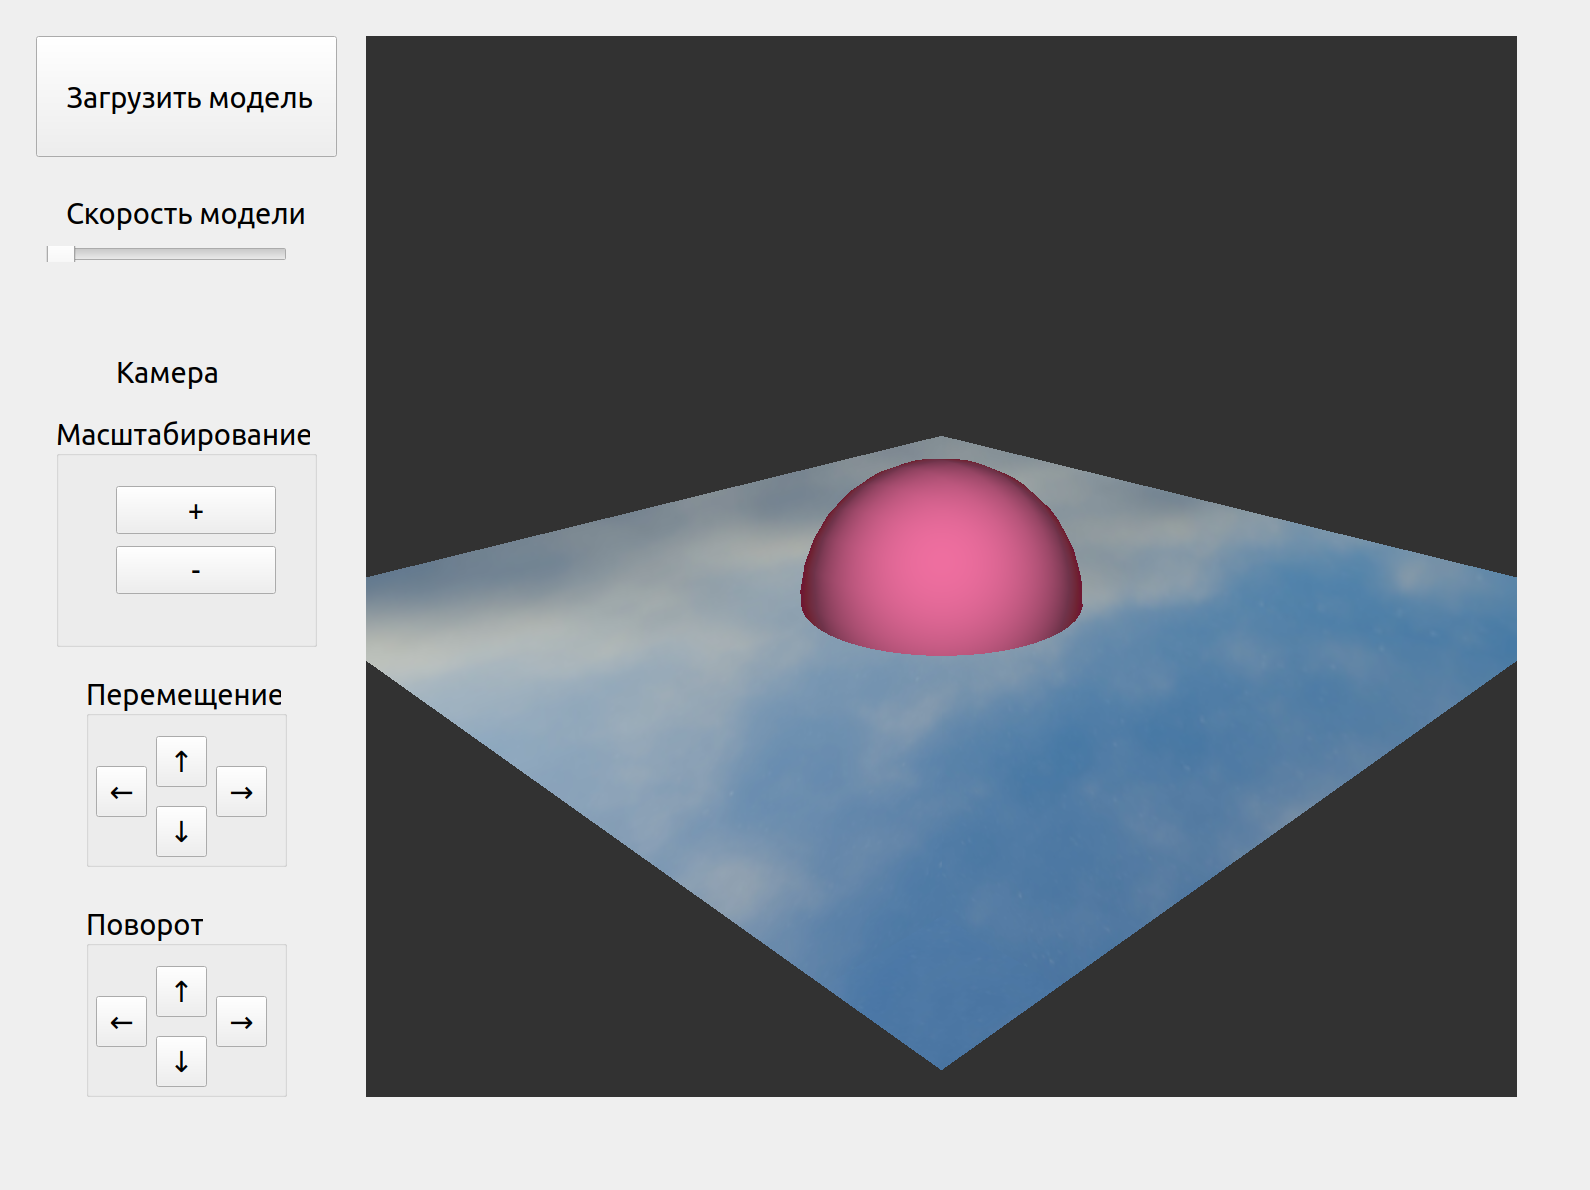
\includegraphics[scale=0.25]{img/example-start.png}
	\end{center}
	\captionsetup{justification=centering}
	\caption{Пример волновой поверхности в положении равновесия}
	\label{img:example-start}
\end{figure}

\begin{figure}[H]
	\begin{center}
		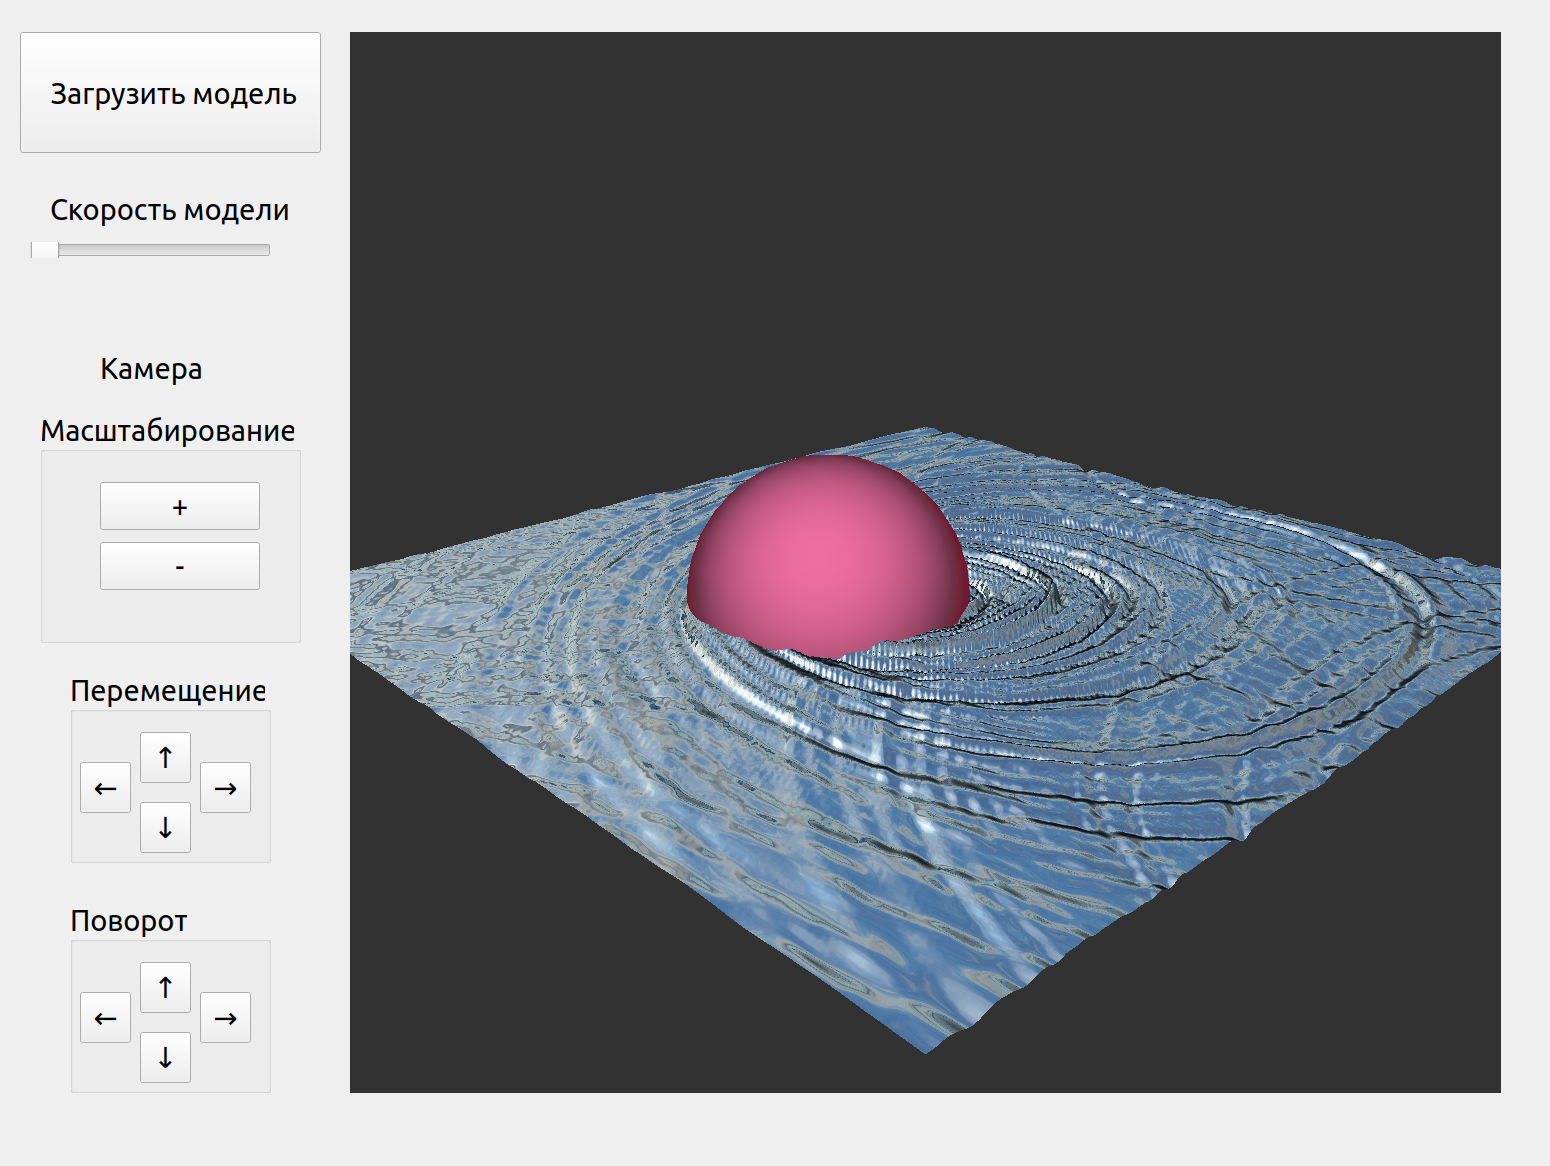
\includegraphics[scale=0.25]{img/example-first.png}
	\end{center}
	\captionsetup{justification=centering}
	\caption{Пример образования волн при движении сферы (вид 1)}
	\label{img:example-first}
\end{figure}

\begin{figure}[H]
	\begin{center}
		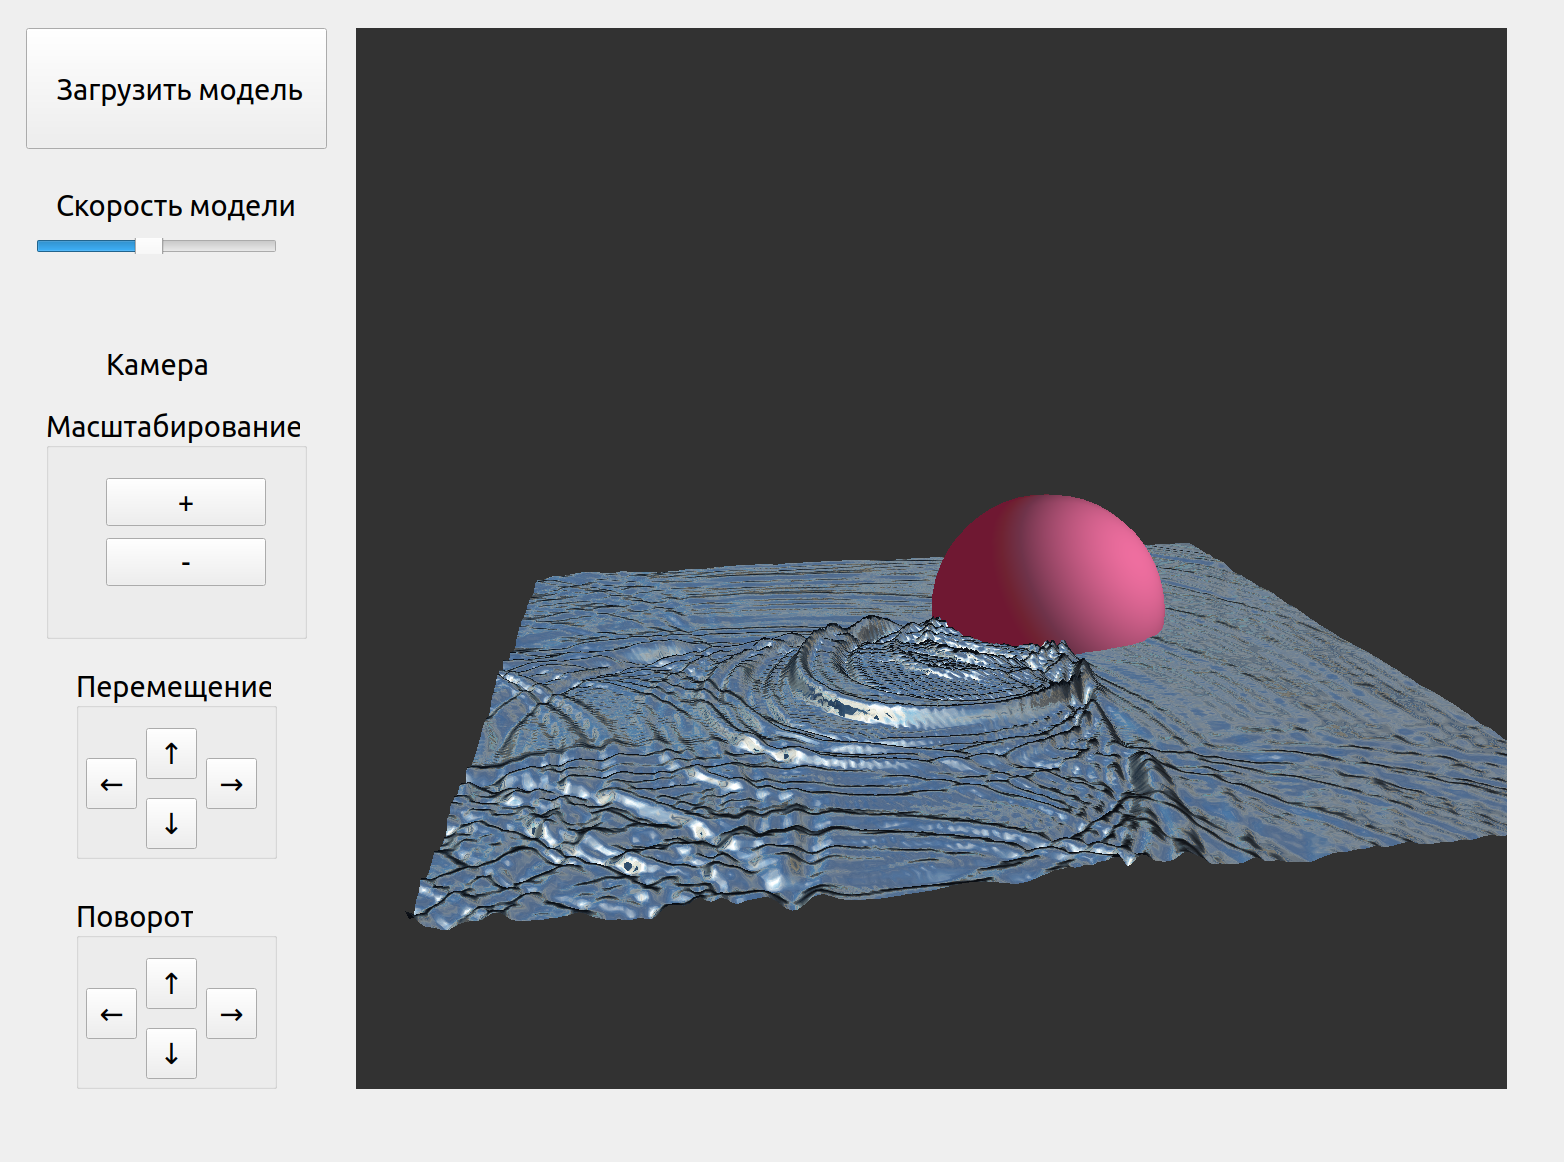
\includegraphics[scale=0.25]{img/example-second.png}
	\end{center}
	\captionsetup{justification=centering}
	\caption{Пример образования волн при движении сферы (вид 2)}
	\label{img:example-second}
\end{figure}

\begin{figure}[H]
	\begin{center}
		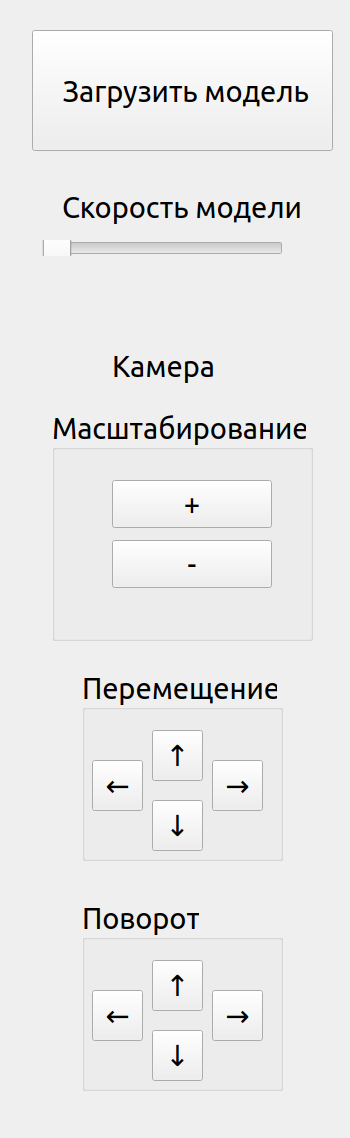
\includegraphics[scale=0.3]{img/control-panel.png}
	\end{center}
	\captionsetup{justification=centering}
	\caption{Окно панели управления}
	\label{img:control-panel}
\end{figure}

\section{Постановка эксперимента}

Метод моделирования оценивают по его скорости выполнения. Количественную характеристику скорости выполнения функций программного обеспечения называют его производительностью.

\subsection{Цель эксперимента}

Целью эксперимента является проведение замеров производительности при создании сцен различной нагруженности. Так как при моделировании волн методом поля высоты поверхность воды представляется сеткой, то параметр, изменяющий нагрузку --- число точек сетки.

Мерой измерения производительности является число кадров в секунду, соответствующее параметру нагрузки. 

При проведении эксперимента скорость движения предмета должна быть одинаковой для каждого числа точек сетки.

\subsection{Технические характеристики}

Тестирование проводилось на устройстве со следующими техническими характеристиками:

\begin{itemize}
	\item операционная система: Ubuntu 20.04.1 Linux x86\_64 \cite{linux};
	\item память : 8 GiB;
	\item процессор: AMD® Ryzen™ 3 3200u @ 2.6 GHz \cite{amd};
	\item видеокарта: Radeon™ Vega 3 Graphics \cite{amd}.
\end{itemize}

Тестирование проводилось на ноутбуке, включенном в сеть электропитания. Во время тестирования ноутбук был нагружен только встроенными приложениями окружения, а также непосредственно системой тестирования.

\subsection{Результаты эксперимента}

Результаты эксперимента приведены в таблице \ref{tab:test}. На рисунке \ref{img:test} представлен график зависимости производительности программного обеспечения от числа точек сетки.

\begin{table}[h]
    \caption{Зависимость производительности программного обеспечения от числа точек сетки}
    \begin{center}
        \begin{tabular}{|l|l|}
            \hline
            Число точек сетки, шт. & Производительность, к/с \\ \hline
            800 & 78 \\ \hline
		    900 & 74 \\ \hline
            1000 & 61 \\ \hline
            1100 & 48 \\ \hline
            1200 & 41 \\ \hline
            1300 & 35 \\ \hline
            1400 & 32 \\ \hline
            1500 & 27 \\ \hline
            1600 & 23 \\ \hline
            1700 & 21 \\ \hline
            1800 & 19 \\ \hline
            1900 & 17 \\ \hline
            2000 & 15 \\ \hline
        \end{tabular}
    \end{center}
    \label{tab:test}
\end{table}

\begin{figure}[H]
	\begin{center}
		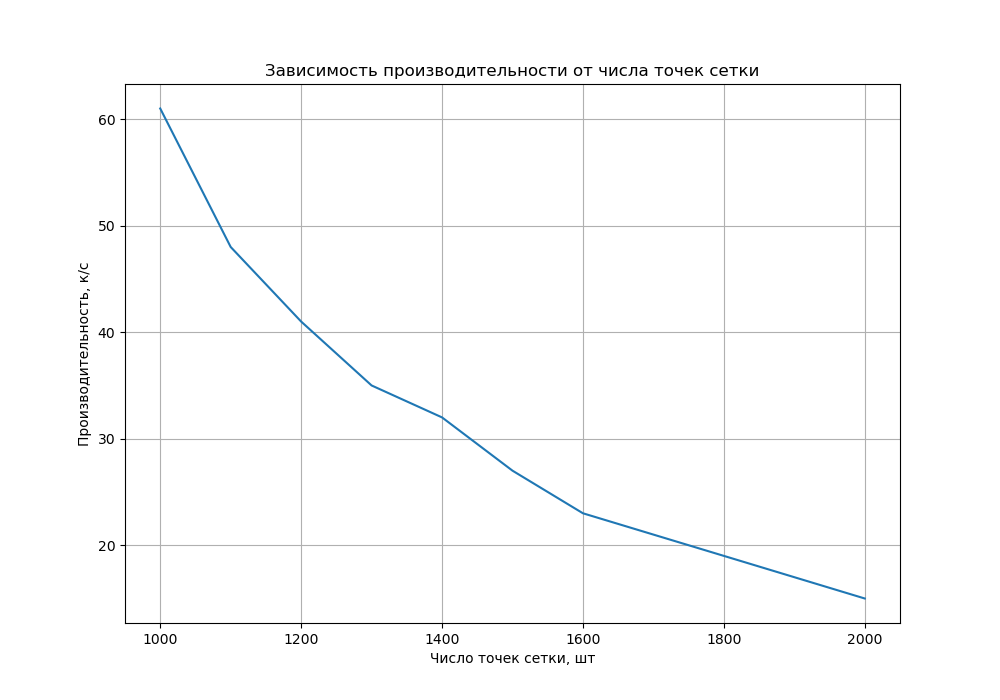
\includegraphics[scale=0.6]{img/test.png}
	\end{center}
	\captionsetup{justification=centering}
	\caption{График зависимости производительности программного обеспечения от числа точек сетки}
	\label{img:test}
\end{figure}

В результате эксперимента получено, что при линейном увеличении числа точек сетки водной поверхности число кадров в секунду экспоненциально уменьшается. 

Для комфортной работы кадровая частота должна быть 60 кадров в секунду \cite{fps}. На графике зависимости производительности от числа точек сетки видно, что оптимальное число точек сетки равняется 1008 штукам.

\section*{Вывод}

Были приведены примеры работы программного обеспечения. Был проведен анализ производительности программного продукта, в результате которого было выяснено, что при линейном увеличении нагрузки на программное обеспечение, его производительность экспоненциально уменьшается.